% Options for packages loaded elsewhere
\PassOptionsToPackage{unicode}{hyperref}
\PassOptionsToPackage{hyphens}{url}
%
\documentclass[
  man,floatsintext]{apa6}
\usepackage{amsmath,amssymb}
\usepackage{lmodern}
\usepackage{iftex}
\ifPDFTeX
  \usepackage[T1]{fontenc}
  \usepackage[utf8]{inputenc}
  \usepackage{textcomp} % provide euro and other symbols
\else % if luatex or xetex
  \usepackage{unicode-math}
  \defaultfontfeatures{Scale=MatchLowercase}
  \defaultfontfeatures[\rmfamily]{Ligatures=TeX,Scale=1}
\fi
% Use upquote if available, for straight quotes in verbatim environments
\IfFileExists{upquote.sty}{\usepackage{upquote}}{}
\IfFileExists{microtype.sty}{% use microtype if available
  \usepackage[]{microtype}
  \UseMicrotypeSet[protrusion]{basicmath} % disable protrusion for tt fonts
}{}
\makeatletter
\@ifundefined{KOMAClassName}{% if non-KOMA class
  \IfFileExists{parskip.sty}{%
    \usepackage{parskip}
  }{% else
    \setlength{\parindent}{0pt}
    \setlength{\parskip}{6pt plus 2pt minus 1pt}}
}{% if KOMA class
  \KOMAoptions{parskip=half}}
\makeatother
\usepackage{xcolor}
\usepackage{graphicx}
\makeatletter
\def\maxwidth{\ifdim\Gin@nat@width>\linewidth\linewidth\else\Gin@nat@width\fi}
\def\maxheight{\ifdim\Gin@nat@height>\textheight\textheight\else\Gin@nat@height\fi}
\makeatother
% Scale images if necessary, so that they will not overflow the page
% margins by default, and it is still possible to overwrite the defaults
% using explicit options in \includegraphics[width, height, ...]{}
\setkeys{Gin}{width=\maxwidth,height=\maxheight,keepaspectratio}
% Set default figure placement to htbp
\makeatletter
\def\fps@figure{htbp}
\makeatother
\setlength{\emergencystretch}{3em} % prevent overfull lines
\providecommand{\tightlist}{%
  \setlength{\itemsep}{0pt}\setlength{\parskip}{0pt}}
\setcounter{secnumdepth}{-\maxdimen} % remove section numbering
% Make \paragraph and \subparagraph free-standing
\ifx\paragraph\undefined\else
  \let\oldparagraph\paragraph
  \renewcommand{\paragraph}[1]{\oldparagraph{#1}\mbox{}}
\fi
\ifx\subparagraph\undefined\else
  \let\oldsubparagraph\subparagraph
  \renewcommand{\subparagraph}[1]{\oldsubparagraph{#1}\mbox{}}
\fi
\newlength{\cslhangindent}
\setlength{\cslhangindent}{1.5em}
\newlength{\csllabelwidth}
\setlength{\csllabelwidth}{3em}
\newlength{\cslentryspacingunit} % times entry-spacing
\setlength{\cslentryspacingunit}{\parskip}
\newenvironment{CSLReferences}[2] % #1 hanging-ident, #2 entry spacing
 {% don't indent paragraphs
  \setlength{\parindent}{0pt}
  % turn on hanging indent if param 1 is 1
  \ifodd #1
  \let\oldpar\par
  \def\par{\hangindent=\cslhangindent\oldpar}
  \fi
  % set entry spacing
  \setlength{\parskip}{#2\cslentryspacingunit}
 }%
 {}
\usepackage{calc}
\newcommand{\CSLBlock}[1]{#1\hfill\break}
\newcommand{\CSLLeftMargin}[1]{\parbox[t]{\csllabelwidth}{#1}}
\newcommand{\CSLRightInline}[1]{\parbox[t]{\linewidth - \csllabelwidth}{#1}\break}
\newcommand{\CSLIndent}[1]{\hspace{\cslhangindent}#1}
\ifLuaTeX
\usepackage[bidi=basic]{babel}
\else
\usepackage[bidi=default]{babel}
\fi
\babelprovide[main,import]{english}
% get rid of language-specific shorthands (see #6817):
\let\LanguageShortHands\languageshorthands
\def\languageshorthands#1{}
% Manuscript styling
\usepackage{upgreek}
\captionsetup{font=singlespacing,justification=justified}

% Table formatting
\usepackage{longtable}
\usepackage{lscape}
% \usepackage[counterclockwise]{rotating}   % Landscape page setup for large tables
\usepackage{multirow}		% Table styling
\usepackage{tabularx}		% Control Column width
\usepackage[flushleft]{threeparttable}	% Allows for three part tables with a specified notes section
\usepackage{threeparttablex}            % Lets threeparttable work with longtable

% Create new environments so endfloat can handle them
% \newenvironment{ltable}
%   {\begin{landscape}\centering\begin{threeparttable}}
%   {\end{threeparttable}\end{landscape}}
\newenvironment{lltable}{\begin{landscape}\centering\begin{ThreePartTable}}{\end{ThreePartTable}\end{landscape}}

% Enables adjusting longtable caption width to table width
% Solution found at http://golatex.de/longtable-mit-caption-so-breit-wie-die-tabelle-t15767.html
\makeatletter
\newcommand\LastLTentrywidth{1em}
\newlength\longtablewidth
\setlength{\longtablewidth}{1in}
\newcommand{\getlongtablewidth}{\begingroup \ifcsname LT@\roman{LT@tables}\endcsname \global\longtablewidth=0pt \renewcommand{\LT@entry}[2]{\global\advance\longtablewidth by ##2\relax\gdef\LastLTentrywidth{##2}}\@nameuse{LT@\roman{LT@tables}} \fi \endgroup}

% \setlength{\parindent}{0.5in}
% \setlength{\parskip}{0pt plus 0pt minus 0pt}

% Overwrite redefinition of paragraph and subparagraph by the default LaTeX template
% See https://github.com/crsh/papaja/issues/292
\makeatletter
\renewcommand{\paragraph}{\@startsection{paragraph}{4}{\parindent}%
  {0\baselineskip \@plus 0.2ex \@minus 0.2ex}%
  {-1em}%
  {\normalfont\normalsize\bfseries\itshape\typesectitle}}

\renewcommand{\subparagraph}[1]{\@startsection{subparagraph}{5}{1em}%
  {0\baselineskip \@plus 0.2ex \@minus 0.2ex}%
  {-\z@\relax}%
  {\normalfont\normalsize\itshape\hspace{\parindent}{#1}\textit{\addperi}}{\relax}}
\makeatother

% \usepackage{etoolbox}
\makeatletter
\patchcmd{\HyOrg@maketitle}
  {\section{\normalfont\normalsize\abstractname}}
  {\section*{\normalfont\normalsize\abstractname}}
  {}{\typeout{Failed to patch abstract.}}
\patchcmd{\HyOrg@maketitle}
  {\section{\protect\normalfont{\@title}}}
  {\section*{\protect\normalfont{\@title}}}
  {}{\typeout{Failed to patch title.}}
\makeatother

\usepackage{xpatch}
\makeatletter
\xapptocmd\appendix
  {\xapptocmd\section
    {\addcontentsline{toc}{section}{\appendixname\ifoneappendix\else~\theappendix\fi\\: #1}}
    {}{\InnerPatchFailed}%
  }
{}{\PatchFailed}
\keywords{keywords\newline\indent Word count: X}
\usepackage{lineno}

\linenumbers
\usepackage{csquotes}
\ifLuaTeX
  \usepackage{selnolig}  % disable illegal ligatures
\fi
\IfFileExists{bookmark.sty}{\usepackage{bookmark}}{\usepackage{hyperref}}
\IfFileExists{xurl.sty}{\usepackage{xurl}}{} % add URL line breaks if available
\urlstyle{same} % disable monospaced font for URLs
\hypersetup{
  pdftitle={Language Input to Blind Infants/Toddlers},
  pdfauthor={Erin Campbell1, Lillianna Righter1, Genia Lukin1, \& Elika Bergelson1},
  pdflang={en-EN},
  pdfkeywords={keywords},
  hidelinks,
  pdfcreator={LaTeX via pandoc}}

\title{Language Input to Blind Infants/Toddlers}
\author{Erin Campbell\textsuperscript{1}, Lillianna Righter\textsuperscript{1}, Genia Lukin\textsuperscript{1}, \& Elika Bergelson\textsuperscript{1}}
\date{}


\shorttitle{Language Input to Blind Infants/Toddlers}

\authornote{

Correspondence concerning this article should be addressed to Erin Campbell, 417 Chapel Drive, Box 90086, Durham, NC 27708. E-mail: \href{mailto:erin.e.campbell@duke.edu}{\nolinkurl{erin.e.campbell@duke.edu}}

}

\affiliation{\vspace{0.5cm}\textsuperscript{1} Department of Psychology \& Neuroscience, Duke University, Durham, NC}

\note{

\textbf{Conflicts of Interest}: The authors have no conflicts of interest to report.
\textbf{Funding}: This work was supported by the National Science Foundation CAREER grant (BCS-1844710) to EB and Graduate Research Fellowship (2019274952) to EC.

}

\begin{document}
\maketitle

\hypertarget{introduction}{%
\section{Introduction}\label{introduction}}

The early language skills of blind children are highly variable (\textbf{campbellsubmitted?}), with some blind children demonstrating age-appropriate vocabulary from the earliest stages of language learning (Bigelow, 1987; Landau \& Gleitman, 1985), while others experience large and persistent language delays (\textbf{CITE?}). Canonically, blind adults become competent speakers of their language and are even reported to have faster language processing skills than their sighted peers (Röder, Demuth, Streb, \& Rösler, 2003; Röder, Rösler, \& Neville, 2000). The causes of this variability and the later ability to ``catch up'' remain poorly understood. In particular, the higher incidence of severe language delays in blind children yields questions about the process of language development in the absence of visual perception: what makes the language learning problem different and apparently more difficult for the blind child? There are multiple possible contributors, including characteristics of the child (e.g., visual acuity, comorbid conditions, gender) as well as characteristics of the environment (e.g., access to early intervention services; school setting; caretakers tailoring interactions to their child's sensory access). Here, we explore the characteristics of the language environment of blind children as it compares to the language environment of their sighted peers. In doing so, we begin to narrow down the role that visual input plays in language development, among all other factors.

Among both typically-developing children and children with developmental differences, language input can predict variability in language outcomes (Anderson, Graham, Prime, Jenkins, \& Madigan, 2021, 2021; Gilkerson et al., 2018; Huttenlocher, Haight, Bryk, Seltzer, \& Lyons, 1991; Huttenlocher, Waterfall, Vasilyeva, Vevea, \& Hedges, 2010; Rowe, 2008, 2012). There are many ways to operationalize language input, that tend to be grouped into \textbf{quantity of language input} and \textbf{input characteristics} (often discussed as \textbf{quality of language input}, c.f. MacLeod and Demers (2023)). Quantity of language input can be broadly construed as the number of words or utterances a child is exposed to. At a coarse level, children who are exposed to more speech (or sign, Watkins, Pittman, \& Walden, 1998) tend to have better language outcomes (Anderson et al., 2021; Gilkerson et al., 2018; Huttenlocher et al., 1991; Rowe, 2008). However, if only the \emph{amount} of language exposure mattered, then infants should be able to sit in front of the television all day and become fluent language users. Yet young children struggle to learn language from video alone (e.g., Roseberry, Hirsh-Pasek, \& Golinkoff, 2014 May-Jun).

The specific characteristics of that language input are perhaps even more important (Hirsh-Pasek et al., 2015; Rowe, 2012), although it is somewhat trickier to turn the qualitative characteristics of language input into operationalizable properties. In this analysis, we move away from describing these linguistic characteristics as ``quality'' measures{[}\^{}1{]}. Rowe and Snow (Rowe \& Snow, 2020) divide this space into three dimensions of language input: interactive features (e.g., parent responsiveness, speech directed \emph{to} child vs.~overheard; conversational turn-taking), linguistic features (e.g., lexical diversity, grammatical complexity), and conceptual features (e.g., topic diversity). These environmental features at various stages interact with the child's own cognitive, linguistic, and conceptual abilities.

{[}\^{}1{]} In the field thus far, the directionality of the term ``quality'' has favored the types of language used by white and abled groups as immutable universal standards, thereby framing racialized and disabled peoples' language as deficit and ``low quality'' by nature. Describing a singular source of input variation as ``high quality'' ignores the sociocultural variation of talk styles, and the presence of many rich sources of information that children can learn from (MacLeod \& Demers, 2023).

An important social feature of the language environment is the amount of interactivity in parent-child communication. Prior literature reports that back-and-forth communicative exchanges (also known as conversational turns) between caregivers and children predict better language learning across infancy (Donnellan, Bannard, McGillion, Slocombe, \& Matthews, 2020; Goldstein \& Schwade, 2008) and toddlerhood (Hirsh-Pasek et al., 2015; Romeo et al., 2018), indicating that parents' active response to their children's actions and utterances supports their learning. Adults' attunement to children's non-linguistic cues of attention and interest, like pointing or eye gaze, also contributes to interactivity. In infancy, words heard in contexts where the adult and child share joint attention are more likely to be learned (Lucca \& Wilbourn, 2018; Tomasello \& Farrar, 1986). Parents' interaction with their child and the world around them ties together the linguistic and conceptual characteristics of the language input, to which we turn next.

Two commonly-analyzed linguistic features are lexical diversity (often measured as type/token ratio) and syntactic complexity. In accounts of the development of sighted children, lexical diversity of language input seems to exert different effects as children get older. In early infancy, children who are exposed to more repetitions (and therefore less lexical diversity) at 7 months have higher vocabulary at age 2 (Newman, Rowe, \& Bernstein Ratner, 2016). This relationship later flips: toddlers who are exposed to greater diversity of words in their language input tend to have larger vocabulary scores (Anderson et al., 2021; Hsu, Hadley, \& Rispoli, 2017; Huttenlocher et al., 2010; Rowe, 2012; Weizman \& Snow, 2001). Lexical diversity is intertwined with input quantity: parents who talk more also tend to provide more lexical diversity (Hoff \& Naigles, 2002 Mar-Apr). Likewise, the diversity of syntactic constructions in parental language input is associated both with children's vocabulary growth and structure diversity in their own productions (De Villiers, 1985; Hadley et al., 2017; Hoff, 2003 Sep-Oct; Huttenlocher, Vasilyeva, Cymerman, \& Levine, 2002; Huttenlocher et al., 2010; Naigles \& Hoff-Ginsberg, 1998).

The conceptual dimension of language input aims to capture the extent to which the language signal maps onto objects and events in the world, which may be a noisy and somewhat opaque connection even with visual input {[}CITE{]}. As with the other dimensions, the pieces of the conceptual content of language input that are most informative may shift across developmental time: as children develop, their ability to represent abstract, displaced, decontextualized referents improves {[}CITE{]}. For example, young infants are more likely to learn a new word when the referent is perceptually salient, dominating their field of view (Yu \& Smith, 2012). Parents responding to a child's point and labeling the object of interest might boost learning in that instance (Lucca \& Wilbourn, 2018). By contrast, \emph{displaced} language use-- that is, talking about past, future, or hypothetical events, or people and items that are not currently present in the environment-- may be beneficial at later stages of development (Rowe, 2013). Indeed, greater decontextualized language use in speech to toddlers predicts kindergarten vocabulary (Rowe, 2012), children's own decontextualized language use (Demir, Rowe, Heller, Goldin-Meadow, \& Levine, 2015), and academic achievement in adolescence (Uccelli, Demir-Lira, Rowe, Levine, \& Goldin-Meadow, 2019). Decontextualized language may support language learning because it provides an opportunity to discuss a broader range of topics and reflects typical adult language usage, which is often abstract (\textbf{CITE?}). It also provides the opportunity for more lexical and syntactic diversity.

From this review, it appears that sighted children learn about the world and language simultaneously from many sources, including sensory perception, linguistic input, and conceptual and social knowledge. For blind children, however, language input may constitute a greater proportion of the available clues for learning than for sighted children; in the absence of visual input, language is an important source of information about the world (E. E. Campbell \& Bergelson, 2022). Syntactic structure provides cues to word meaning that may be lost without visual cues, such as the relationship between two entities that aren't within reach (\textbf{gleitman1990?}). In our review so far, we have presented a pattern wherein the features of the input that are most helpful for language learning change over the course of children's development: early on, many of these cues require visual access,such as parental gaze, shared visual attention, pointing to remote object and the presence of salient objects in the visual field. Only later in development do the handholds to language learning become more abstract. This may be part of the reason why language delays are common in blind toddlers, but often resolved in older childhood {[}CITE{]}. If direct sensory access is the key to unlocking the meaning of early words, it may take longer to gain enough environmental experience to make early language learning strides-- that is, it may take longer in infancy to build a ``semantic seed'' (\textbf{babineau2021?}; \textbf{babineau2022?}). By hypothesis, once this initial seed of linguistic knowledge is acquired, blind children and sighted children alike are able to use more abstract and linguistic features as cues, and learning proceeds rapidly (E. E. Campbell \& Bergelson, 2022). Nevertheless, we cannot assume that access to visual experience is the \emph{only} difference in the language learning experiences for blind and sighted children. The language input itself may very well differ for blind children relative to sighted children, for a variety of reasons.

First, speakers regularly tailor input to communicate efficiently with the listener (\textbf{grice1975?}). Parents are sensitive to their child's developmental level and tune language input accordingly (Snow, 1972; Vygotsky \& Cole, 1978). Child-directed speech is one example--whereby parents speak to young children with exaggerated prosody, slower speech rate, and increased vowel clarity (Bernstein Ratner, 1984; Fernald, 1989), which is in some cases helpful to the young language learner (Thiessen, Hill, \& Saffran, 2005). Parents show increased alignment (a tendency to re-use the conversation partner's expressions) for younger children, which decreases as children get older (Yurovsky, Doyle, \& Frank, 2016). When interacting with infants and toddlers, parents repeat words more often than when interacting with older children or adults (Snow, 1972). Communicative tailoring is also common in language input to children with disabilities, who tend to receive simplified, more directive language input, and less interactive input compared to typically-developing children (Dirks, Stevens, Kok, Frijns, \& Rieffe, 2020; Yoshinaga-Itano, Sedey, Mason, Wiggin, \& Chung, 2020).

In addition to tailoring communication to children's developmental level, speakers also adjust their conversation in accordance with the conversation partner's sensory access (Gergle, Kraut, \& Fussell, 2004; Grigoroglou, Edu, \& Papafragou, 2016). In a noisy environment, speakers will adapt the acoustic-phonetic features of their speech with the intent to make it easier for their interlocutor to understand them (Hazan \& Baker, 2011), which demonstrates sensitivity to even temporary sensory conditions of their conversation partner. When describing scenes, speakers aim to provide the information their listeners lack but avoid redundant visual description (Ostarek, Paridon, \& Montero-Melis, 2019; \textbf{grice1975?}). During in-lab tasks with sighted participants, participants tailor their descriptions and requests by verbally providing visually-absent cues when an object is occluded to their partner (Hawkins, Gweon, \& Goodman, 2021; Jara-Ettinger \& Rubio-Fernandez, 2021; Rubio-Fernandez, 2019). These results suggest that adults and even infants (Chiesa, Galati, \& Schmidt, 2015; Ganea et al., 2018; Senju et al., 2013) can flexibly adapt communication to the visual and auditory abilities of their partner.

Curiously though, these patterns are not borne out in the existing literature on interactions between blind infants and their sighted parents. We might expect parents to verbally compensate for missing visual input, resulting in parents providing more description of the child's environment. Instead, caregivers of blind children seem to restrict conversation to things that the blind child is currently engaged with, rather than attempt to redirect their attention to other stimuli (Andersen, Dunlea, \& Kekelis, 1993; J. Campbell, 2003; Kekelis \& Andersen, 1984). In naturalistic settings, parents of blind children use \emph{fewer} declaratives and \emph{more} imperatives than parents of sighted children, suggesting that children might be receiving less description than sighted children (Kekelis \& Andersen, 1984; Landau \& Gleitman, 1985). On the other hand, some parents may adapt to their children's visual abilities in specific contexts. Tadić, Pring, and Dale (2013 Nov-Dec) and colleagues find that in a structured book reading task, parents of blind children provide more descriptive utterances than parents of sighted children. Further, parents of blind children provide more tactile cues to initiate interactions or establish joint attention (Preisler, 1991; Urwin, 1983), which may serve the same social role as shared gaze in sighted children. These mixed results suggest that parents of blind children might alter language input in some domains but not others.

Better understanding how sensory perception and linguistic input interact to influence blind children's language outcomes is of great clinical and scientific importance. Based on our own interactions with participants' families in the present study, parents are looking for evidence-based guidance to help them support their children's language development. If properties of language input influence the likelihood of language delays among blind infants and toddlers (\textbf{campbellsubmitted?}), capturing this variation may reveal a more nuanced picture of how infants use the input to learn language. By contrast, if there is no relationship between language input properties and children's language outcomes, then trying to modify language input can be one less worry for caregivers. In the present study, we examine daylong recordings of the naturalistic language environments of blind and sighted children in order to characterize the input to each group. We first measure input quantity (adult word count) and analyze several characteristics that may be information-rich learning cues, including interactivity( conversational turn counts, proportion of child-directed speech), conceptual features (temporal displacement, sensory modality), and linguistic complexity (type/token ratio and mean length of utterance). We then link these properties of language input to language outcomes and explore whether the effects vary as a function of children's perceptual ability.

\hypertarget{methods}{%
\section{Methods}\label{methods}}

\hypertarget{participants}{%
\subsection{Participants}\label{participants}}

29 blind infants and their families participated in this study. Blind participants were recruited through opthamologist referral, preschools, early intervention programs, social media, and word of mouth. To be eligible for this study, participants had to be 6--30 months old, have no additional disabilities (developmental delays; intellectual disabilities, or hearing loss), and be exposed to \(\geq\) 75\% English at home. Given the wide age range of the study, to control for age, each blind participant was matched to a sighted partcipicant, based on age (\(\pm\) 6 weeks), gender, maternal education (\(\pm\) one education level: less than high school diploma, high school diploma, some college / Associate's, Bachelor's, graduate school), and number of siblings (\(\pm\) 1 sibling). When more than one match was available, we prioritized matching the blind participants as closely as possible on each characteristic in the preceding order. Caregivers were asked to complete a demographics survey and the MacArthur-Bates Communicative Development Inventory (CDI, Fenson et al., 1994) within one week of the home language recording. See Table @ref(tab: participant-characteristics) for sample characteristics.

\% latex table generated in R 4.2.1 by xtable 1.8-4 package
\% Fri Apr 21 17:03:27 2023

\begin{table}[ht]
\centering
\begin{tabular}{lrrr}
  \hline
Variable & Blind & Sighted & Overall \\ 
  \hline
\vspace*{0.1cm} \\ \textbf{Age in months      } &  &  &  \\ 
  \hskip .5cm    Mean (SD) & 15.77 (8.20) & 16.15 (8.15) & 15.96 (8.04) \\ 
  \hskip .5cm    Min, Max & 6.41, 30.38 & 6.18, 31.76 & 6.18, 31.76 \\ 
  \hskip .5cm \textbf{ } &   &   &   \\ 
  \vspace*{0.1cm} \\ \textbf{Gender      } &  &  &  \\ 
  \hskip .5cm   (Col \%) &  &  &  \\ 
  \hskip .5cm \textbf{  F} & 7 (43.75\%) & 7 (43.75\%) & 14 (43.75\%) \\ 
  \hskip .5cm \textbf{  M} & 9 (56.25\%) & 9 (56.25\%) & 18 (56.25\%) \\ 
  \hskip .5cm \textbf{ } &   &   &   \\ 
  \vspace*{0.1cm} \\ \textbf{Maternal education level      } &  &  &  \\ 
  \hskip .5cm   (Col \%) &  &  &  \\ 
  \hskip .5cm \textbf{  Some college} & 0 ( 0.00\%) & 0 ( 0.00\%) & 0 ( 0.00\%) \\ 
  \hskip .5cm \textbf{  Associate's degree} & 3 (23.08\%) & 1 ( 7.69\%) & 4 (15.38\%) \\ 
  \hskip .5cm \textbf{  Bachelor's degree} & 1 ( 7.69\%) & 2 (15.38\%) & 3 (11.54\%) \\ 
  \hskip .5cm \textbf{  Master's degree} & 5 (38.46\%) & 9 (69.23\%) & 14 (53.85\%) \\ 
  \hskip .5cm   Missing & 4 (30.77\%) & 1 ( 7.69\%) & 5 (19.23\%) \\ 
  \vspace*{0.1cm} \\ \textbf{Maternal education level      } & 0 ( 0.00\%) & 0 ( 0.00\%) & 0 ( 0.00\%) \\ 
  \hskip .5cm \textbf{ } &   &   &   \\ 
  \vspace*{0.1cm} \\ \textbf{Number of older siblings      } &  &  &  \\ 
  \hskip .5cm    Mean (SD) & 0.50 (0.82) & 1.09 (1.04) & 0.74 (0.94) \\ 
  \hskip .5cm    Min, Max & 0.00, 2.00 & 0.00, 3.00 & 0.00, 3.00 \\ 
  \hskip .5cm \textbf{ } &   &   &   \\ 
  \vspace*{0.1cm} \\ \textbf{Vision diagnosis      } &  &  &  \\ 
  \hskip .5cm   (Col \%) &  &  &  \\ 
  \hskip .5cm \textbf{  Cataracts} & 3 (18.75\%) & - & 3 (18.75\%) \\ 
  \hskip .5cm \textbf{  Leber's Congenital Amaurosis } & 1 ( 6.25\%) & - & 1 ( 6.25\%) \\ 
  \hskip .5cm \textbf{  Microphthalmia } & 2 (12.50\%) & - & 2 (12.50\%) \\ 
  \hskip .5cm \textbf{  Multiple} & 2 (12.50\%) & - & 2 (12.50\%) \\ 
  \hskip .5cm \textbf{  Not specified} & 2 (12.50\%) & - & 2 (12.50\%) \\ 
  \hskip .5cm \textbf{  Ocular albinism} & 2 (12.50\%) & - & 2 (12.50\%) \\ 
  \hskip .5cm \textbf{  Optic Nerve Hypoplasia} & 2 (12.50\%) & - & 2 (12.50\%) \\ 
  \hskip .5cm \textbf{  Retinal Detachments} & 1 ( 6.25\%) & - & 1 ( 6.25\%) \\ 
  \hskip .5cm \textbf{  Retinopathy of Prematurity} & 1 ( 6.25\%) & - & 1 ( 6.25\%) \\ 
  \hskip .5cm \textbf{ } &   &   &   \\ 
  \vspace*{0.1cm} \\ \textbf{Race      } &  &  &  \\ 
  \hskip .5cm   (Col \%) &  &  &  \\ 
  \hskip .5cm \textbf{  } & 0 ( 0.00\%) & 7 (43.75\%) & 7 (21.88\%) \\ 
  \hskip .5cm \textbf{  American Indian or Alaska Native} & 1 ( 6.25\%) & 0 ( 0.00\%) & 1 ( 3.12\%) \\ 
  \hskip .5cm \textbf{  Black or African American} & 1 ( 6.25\%) & 1 ( 6.25\%) & 2 ( 6.25\%) \\ 
  \hskip .5cm \textbf{  Mixed} & 3 (18.75\%) & 1 ( 6.25\%) & 4 (12.50\%) \\ 
  \hskip .5cm \textbf{  White} & 11 (68.75\%) & 7 (43.75\%) & 18 (56.25\%) \\ 
  \hskip .5cm \textbf{ } &   &   &   \\ 
  \vspace*{0.1cm} \\ \textbf{Ethnicity      } &  &  &  \\ 
  \hskip .5cm   (Col \%) &  &  &  \\ 
  \hskip .5cm \textbf{  } & 0 ( 0.00\%) & 8 (50.00\%) & 8 (25.00\%) \\ 
  \hskip .5cm \textbf{  Hispanic or Latino} & 3 (18.75\%) & 0 ( 0.00\%) & 3 ( 9.38\%) \\ 
  \hskip .5cm \textbf{  Not Hispanic or Latino} & 13 (81.25\%) & 8 (50.00\%) & 21 (65.62\%) \\ 
  \hskip .5cm \textbf{ } &   &   &   \\ 
   \hline
\end{tabular}
\end{table}

\hypertarget{recording-procedure}{%
\subsection{Recording Procedure}\label{recording-procedure}}

Eligible families were asked to complete two surveys and complete a daylong home language recording. For the recording portion of the study, caregivers of participating infants received a LENA wearable audio recorder (Ganek \& Eriks-Brophy, 2016) and vest. They were instructed to place the recorder in the vest on the day of their scheduled recording and put the vest on their child from the time they woke up until the recorder automatically shut off after 16 hours (setting vest nearby during bath, nap, and car times). They were also instructed how to pause the recording at any time, but asked to keep these pauses to a minimum. Actual recording length ranged from 8 hours 17 minutes to 15 hours 59 minutes (15 hours 16 minutes).

\hypertarget{processing}{%
\subsection{Processing}\label{processing}}

Audio recordings were first processed by LENA proprietary software, creating algorithmic measures such as conversational turn counts. Each recording was then run through an in-house automated sampler that selected 15- non-overlapping 5-minute segments, randomly distributed across the duration of the recording. The process output a codeable ELAN file (.eaf, \textbf{brugman2009?}). Each segment consists of 2 core minutes of annotated time, with 2 minutes of listenable context marked out preceding the annotation clip and 1 minute of additional context following the annotation clip. Each file therefore contains 30 minutes of coded recording time and 75 minutes of total time listened. Because these segments were sampled randomly, and not on a high-volubility measure such as conversational turns or adult speech density, the amount of time with codeable speech input varied for each recording. Indeed, across participants roughly 27\% of the random 2-minute coding segments contained no speech at all.

Once the randomly selected segments were annotated, we also chose to annotate 15 additional segments specifically for their high levels of speech. To select these segments of dense talk, we first conducted an automated analysis of the audio file using the voice type classifier for child-centered daylong recordings (Lavechin, Bousbib, Bredin, Dupoux, \& Cristia, 2021) which identified all human speech in the recording. The entire recording was then broken into 2-minute chunks marked out at zero-second timestamps (e.g.~00:02:00.000 to 00:04:00.000). Each of these chunks was then ranked highest to lowest by the total duration of speech contained within the boundaries. For our high volubility sample, we chose the highest-ranked 15 segments of each recording, excluding those that overlapped with already-coded random segments.

\hypertarget{annotation}{%
\subsection{Annotation}\label{annotation}}

Trained annotators listened through each 2-minute segment plus its surrounding context and coded it using the Analyzing Child Language Experiences around the World (ACLEW) Daylong Audio Recording of Children's Linguistic Environments (DARCLE) annotation scheme (Soderstrom et al., 2021). Prior to annotating lab data, annotators are trained on previously coded samples of child recordings and are required to reach 95\% overall agreement with the gold standard version of the file for three different age ranges: 0-7 months, 8-18 months, and 19-36 months. For more information about this annotation scheme and the larger project, please see the ACLEW homepage (\url{https://sites.google.com/view/aclewdid/home}). Following the first pass, all files were by a highly-trained ``superchecker'' to ensure the consistency of annotations.

This annotation scheme is designed to capture both utterances by the target child and speech in the child's environment, including adults, other children, and pre-recorded electronic speech (e.g.~toys, television, the radio). Annotators segment the duration of each utterance on a separate coding tier for each unique speaker (exceptions: all electronic speech is coded on the same tier, and some speakers who appear briefly in these files were not easily distinguishable from others by annotators naive to their identities, so they may be concatenated on the same tier). Speech by people other than the target child is transcribed using an adapted version of CHAT transcription style (MacWhinney, 2019), dubbed minCHAT for the ACLEW project (Soderstrom et al., 2021). Because the majority of target children in the project are pre-lexical or phonetically immature, utterances produced by the target child are not transcribed.

Each utterance is coded for additional linguistic properties from a set of pre-determined categories. Target child utterances are coded for vocal maturity, lexical status, and multi-word status. Vocal maturity classifies utterances into the following categories: laughing; crying; canonical syllables that contain a consonant-like and vowel-like sound component, including both babbling and identifiable words; non-canonical syllables, which do not contain both consonant and vowel portions, or which do not transition between them in a speech-like way; and unsure, when the vocalization type is unclear. Each vocalization that contains canonical syllables is then coded for lexical status (does it contain an identifiable lexical item?). Finally, each utterance with a lexical item is coded for multi-word status (does it contain more than one unique word type?).

Environmental speech from everyone else is coded for the addressee of each utterance: speech directed to a child, whether or not it is directed to the target child; adult-directed speech; speech directed to both an adult and a child; speech directed to pets or other animals; speech with an unclear addressee; or speech directed towards a recipient that doesn't fit into another category (e.g.~voice control of Siri or Alexa, prayer to a metaphysical entity).

\hypertarget{results}{%
\section{Results}\label{results}}

\hypertarget{measuring-properties-of-language-input}{%
\subsection{Measuring Properties of Language Input}\label{measuring-properties-of-language-input}}

We first seek to assess whether language input to blind children is categorically different from the language input to sighted children, along the dimensions of quantity, interactiveness, linguistic properties, and conceptual properties. For continuous variables, we test for group differences using a t-test, and for categorical variables we use Wilcoxon signed rank tests to assess differences in the variables' relative proportion. We use non-parametric versions of these tests when a Shapiro-Wilks test indicates that the variable is not normally distributed. Because this analysis involves multiple tests of the null hypothesis (\emph{that there is no difference in the language input to blind vs.~sighted kids}), we use the conservative Bonferroni correction to set our threshold for significance (\emph{p} = 0.05 / 8 tests = 0.01).

\hypertarget{language-input-quantity}{%
\subsubsection{Language Input Quantity}\label{language-input-quantity}}

We first compare the quantity of language input to blind and sighted children using two measures of the number of words in their environment: LENA's automated Adult Word Count and word token count from our manual annotations. Shapiro-Wilks tests indicated that both of these variables were normally distributed (\emph{p}s \textgreater{} .05).

Turning first to LENA's automated measure, a two-sample t-test shows that despite wide variability in the number of words children hear (Range: 6233--31745 words\textsubscript{blind}, 6027--25500 words\textsubscript{sighted}), blind and sighted children do not differ in language input quantity (\emph{t}(45.26) = -1.99, \emph{p} = .053). If we instead measure this using word counts from the transcriptions of the audio recordings, we find parallel results: blind and sighted children do not differ in language input quantity (\emph{t}(27.00) = 0.08, \emph{p} = .939); see Figure \ref{fig:quantity-plots}.

\begin{figure}
\centering
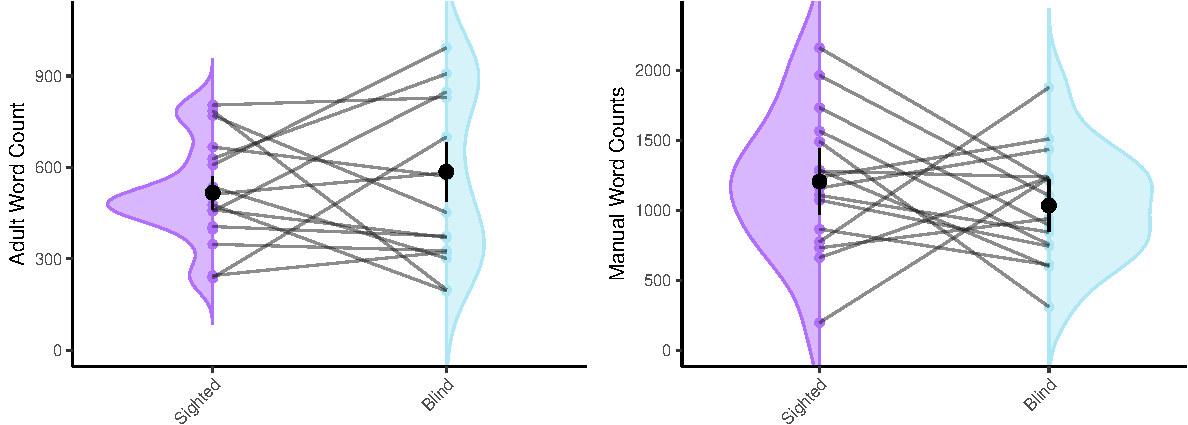
\includegraphics{input_quality_manuscript_files/figure-latex/quantity-plots-1.pdf}
\caption{\label{fig:quantity-plots}Comparing LENA-generated adult word counts (left) and transcription-based word counts in the input of blind and sighted children. Each dot represents the estimated number of words in one child's recording.}
\end{figure}

\hypertarget{interactiveness}{%
\subsubsection{Interactiveness}\label{interactiveness}}

We compared the proportions of child-directed speech (CDS) between the blind children and their sighted matches. Each proportion was calculated as the number of utterances produced by someone \emph{other} than the target child (non-CHI utterances) tagged with a child addressee out of the total number of non-CHI utterances for each sensory group. A two-sample test for equality of proportions revealed no significant difference in the overall proportions of CDS to blind children and CDS to sighted children.

We next compare the number of conversational turn counts for blind and sighted children, using LENA's automated Conversational Turn Count measure. This measure is not normally distributed (W = 0.92, \emph{p} = .924). Despite wide variability in conversational turns (210--1436 \textsubscript{blind}, 112--1348 \textsubscript{sighted}), we find no evidence for group-level differences between blind and sighted children (W = 456, \emph{p} = .585).

\begin{figure}
\centering
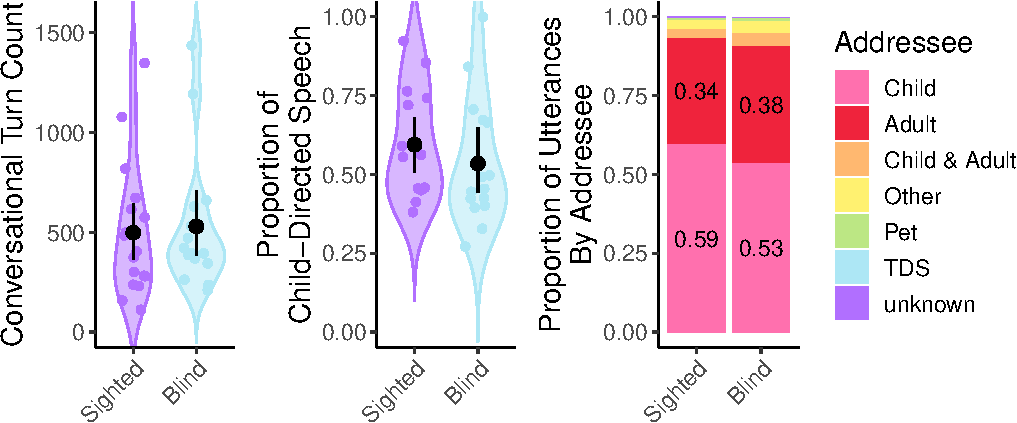
\includegraphics{input_quality_manuscript_files/figure-latex/interactiveness-plots-1.pdf}
\caption{\label{fig:interactiveness-plots}Comparing LENA-generated conversational turn counts (left) and proportion of utterances in child-directed speech (center). Each dot represents one child's recording. The full breakdown by addressee is shown in the rightmost panel.}
\end{figure}

\hypertarget{linguistic-features}{%
\subsubsection{Linguistic Features}\label{linguistic-features}}

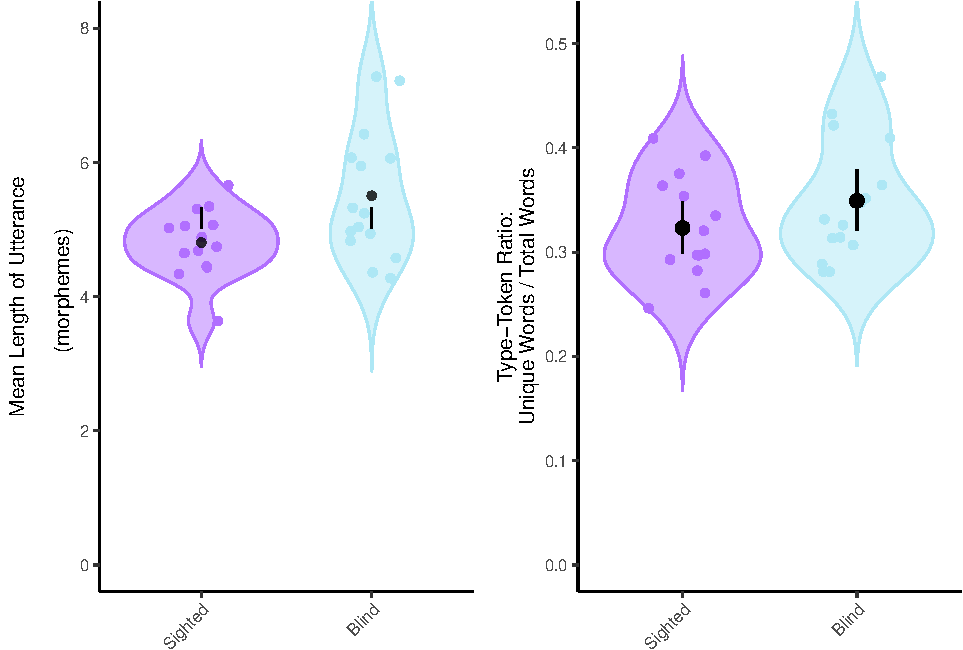
\includegraphics{input_quality_manuscript_files/figure-latex/linguistic-plots-1.pdf}

For linguistic features, we first measure the proportion of unique words divided by the number of total words in the input, or type-token ratio, from the manual annotations. Because this variable met the normality assumption, we performed a two-sample t-test. Results indicated that there was no significant difference in the type-token ratio between the two groups (\emph{t}(26.75) = -1.29, \emph{p} = .208). This suggests that, on average, the type-token ratio is similar for blind (M: 0.35) and sighted (M: 0.32) children (see Figure \ref{fig:TTR}). These results provide evidence that the variety of words in the input is not affected by children's vision.

We also analyzed the syntactic complexity of children's language input, approximated as utterance length in morphemes. Each utterance by a non-CHI speaker was tokenized into morphemes using the `morphemepiece' R package (\textbf{bratt2022?}). We then calculated the mean length of utternace (MLU) per speaker in each audio recording, and then compared the MLU of environmental speech to blind children (M(SD) = 5.08 (1.29)) to that of sighted children (M(SD) = (M(SD) = 4.47 (1.39)); this variable was normally distributed (W = 0.92, \emph{p} = .924). A two-sample t-test revealed that the MLU was slightly but significantly higher in speech to blind children than to their sighted peers (\emph{t}(147.71) = -2.80, \emph{p} = .006).

\hypertarget{conceptual-features}{%
\subsubsection{Conceptual Features}\label{conceptual-features}}

Our analysis of the conceptual features aims to measure whether the extent to which language input centers around the \emph{``here and now''}: objects/events that are currently present/occurring vs.~displaced objects/events. Prior work has quantified such \emph{here-and-now}ness by counting object presence co-occurring with a related noun label {[}CITE{]}. The audio format of our data and the coding scheme we use make it difficult to ascertain object presence, so instead of object displacement, in this analysis, we approximate \emph{here-and-now}ness using lexical and syntactic properties of the input. We do this by comparing 1) What proportion of words are temporally displaced?; 2) To what extent can children physically engage in / interact with words' referents?; and 3) What proportion of words have referents that can only be experienced through vision?

The last conceptual feature we examined is the displacement of events discussed in children's linguistic environment, via properties of the verbs in their input. Notably, we are attempting to highlight semantic features of the language environment; however, given the constraints of large-scale textual analysis, we are categorizing utterances based on a combination of closely related syntactic and morphological features of verbs, since these contain time-relevant information. We recognize that these linguistic features do not perfectly align with the temporal structure of the world. We assigned each utterance a \textbf{temporality} value: utterances tagged \emph{displaced} describe events that take place in the past, future, or irrealis space, while utterances tagged \emph{present} describe current, ongoing events. A small amount of utterances (n = XXX r n\_uncat) were left \emph{uncategorized} because they were fragments or because the automated parser failed to tag any of the relevant features. To do this, we used the udpipe package (\textbf{wijffels2023?}) to tag the transcriptions with parts of speech and other lexical features, such as tense, number agreement, or case inflection. To be marked as present, a verb either had to be marked with both present tense and indicative mood, or appear in the gerund form with no marked tense (e.g.~\emph{you talking to Papa?}). Features that could mark an utterance as displaced included past tense, presence of a modal, presence of \emph{if}, or presence of \emph{gonna}/\emph{going to}, \emph{have to}, \emph{wanna}/\emph{want to}, or \emph{gotta}/\emph{got to}, since these typically indicate belief states and desires, rather than real-time events. In the case of utterances with multiple verbs, we selected the features from the first verb or auxiliary, as a proxy for hierarchical dominance.

We compare the proportion of temporally displaced verbs using a Wilcoxon rank-sum test, given that a Shapiro-Wilks test indicates that the proportion of displaced verbs does not follow a normal distribution (W = 0.98, \emph{p} = .977). We find that blind children hear proportionally more displaced verbs than blind children (\emph{W} = 36.50, \emph{p} = .003).

Next, we measure whether Child-Body-Object Interaction (CBOI) rating (\textbf{muraki2022?}). These norms were generated by asking parents of six-year-olds to rate the extent to which children physically interact with words' referents, from 1 (\emph{things that a typical child does not easily physically interact with}) to 7 (\emph{things a typical child would easily physically interact with}). We first use the udpipe part-of-speech tags to filter to content words (adjectives, adverbs, nouns, and verbs). Words without a CBOI rating (N = XXX/XXX) were removed. We then compared the distribution of CBOI ratings in word tokens in blind children's input to that in sighted children's input using a two-sample Kilgomorov-Smirnov test. We find that these distributions significantly differ (D = 0.98, \emph{p} \textless{} .001) this difference survives Bonferroni correction. Descriptively, low CBOI words were more common in language input to blind children, and high CBOI words were more common in language input to sighted children.

Lastly, we measure whether the language input to blind children contains a different proportion of words referring to visual objects/actions/properties. This is perhaps the dimension that people tend to have the strongest a priori hyptheses about: \emph{Perhaps parents speak less about visual concepts to blind children because they're less relevant to the children's experiences} or alternatively \emph{Perhaps parents speak} more* \emph{about visual concepts, in order to compensate for experiences they perceive their children as missing}. We categorize the perceptual modalities of words' referents using the Lancaster Sensorimotor Norms, ratings from typically-sighted adults about the extent to which a word evokes a visual/tactile/auditory/etc. experience (\textbf{lynott2020?}). Words with higher ratings in a given modality are more strongly associated with perceptual experience in that modality. A word's dominant perceptual modality is the modality which received the highest mean rating. We tweak this categorization in two ways: words which received low ratings (\textless{} 3.5) across all modalities were re-categorized as \emph{amodal}, and words whose ratings were distributed across modalities were re-categorized as \emph{multimodal}. Using this system, each of the content words in children's input (adjectives, adverbs, nouns, and verbs) were categorized into their primary perceptual modality. For each child, we extracted the proportion of ``visual'' words in their language environment; this variable was normally distributed (W = 0.96, \emph{p} = .962). We found no differences across groups in the proportion of highly visual words (\emph{t}(25.11) = 0.32, \emph{p} = .755).

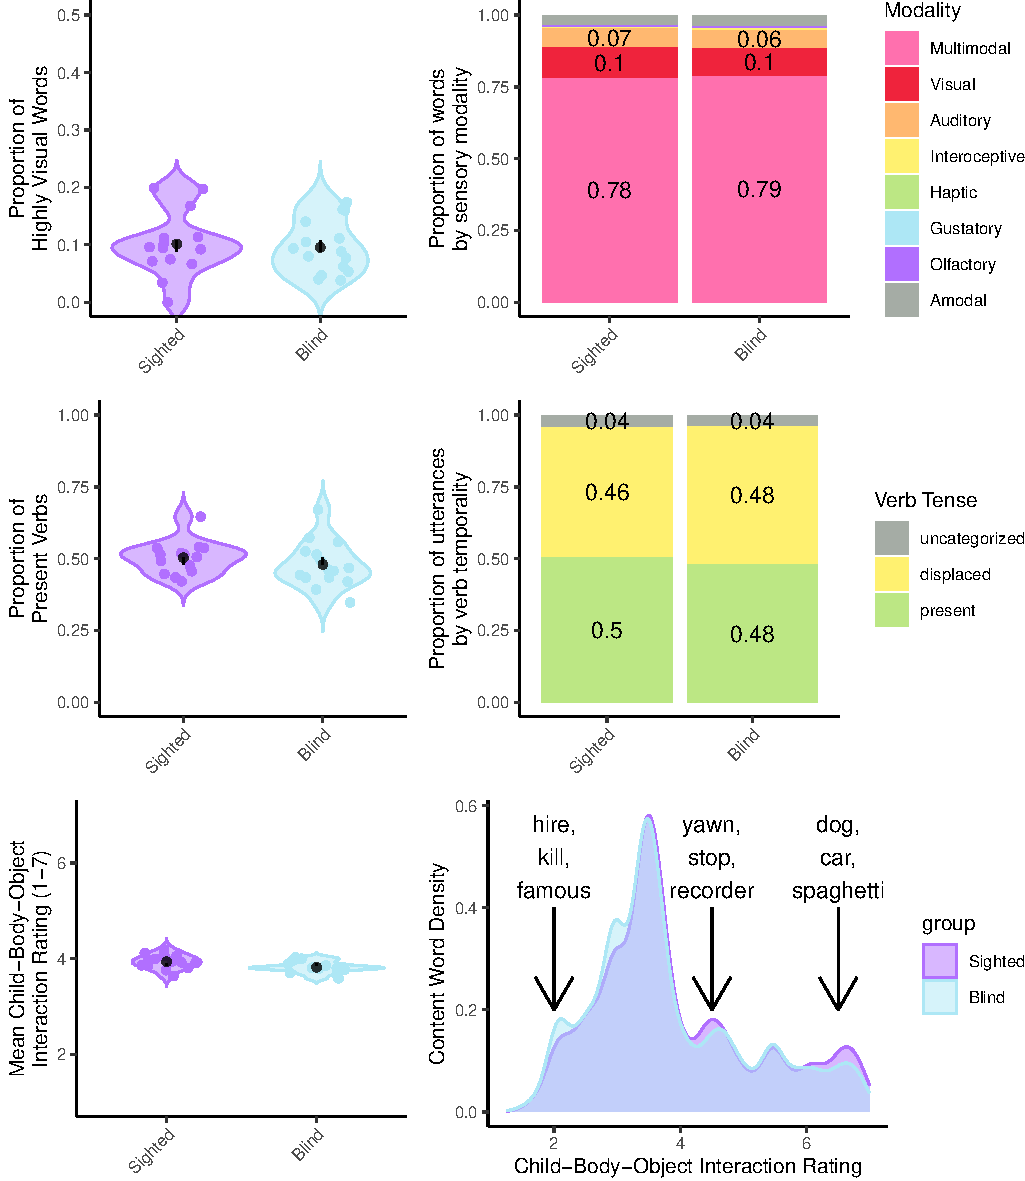
\includegraphics{input_quality_manuscript_files/figure-latex/conceptual-plots-1.pdf}

\hypertarget{patterns-in-language-input}{%
\subsubsection{Patterns in Language Input}\label{patterns-in-language-input}}

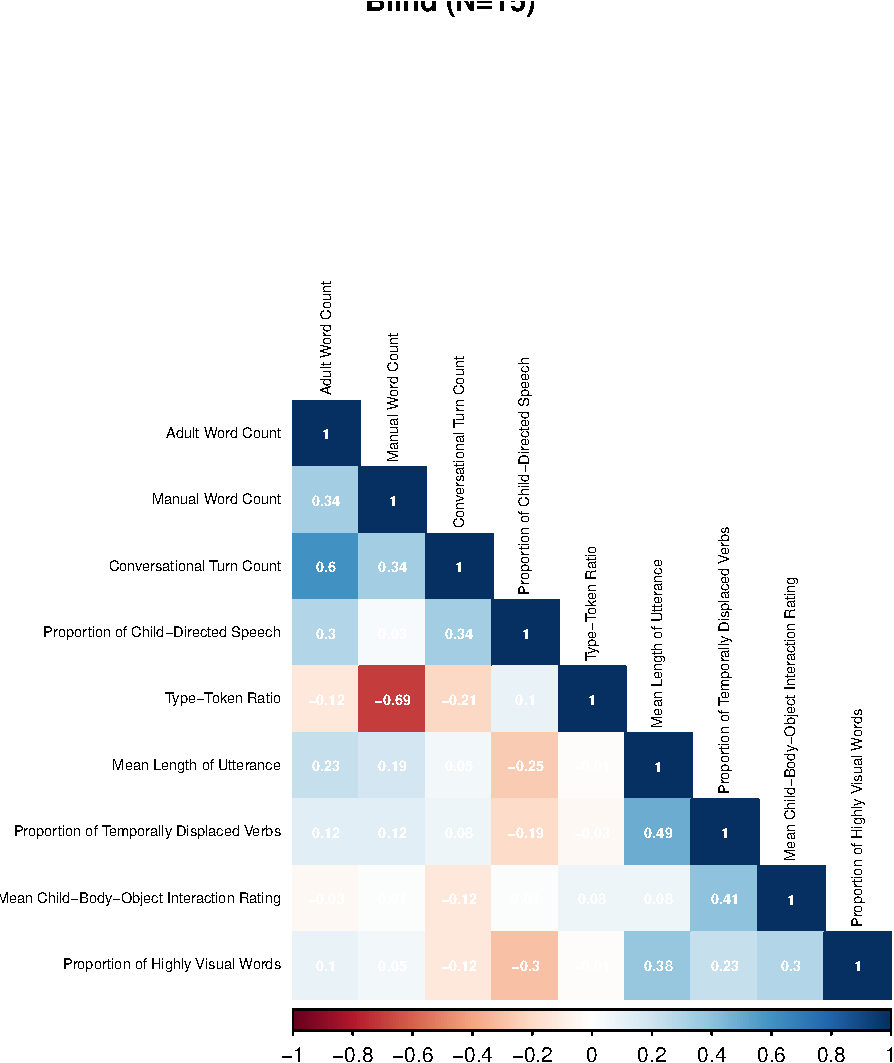
\includegraphics{input_quality_manuscript_files/figure-latex/compare-corrs-1.pdf} 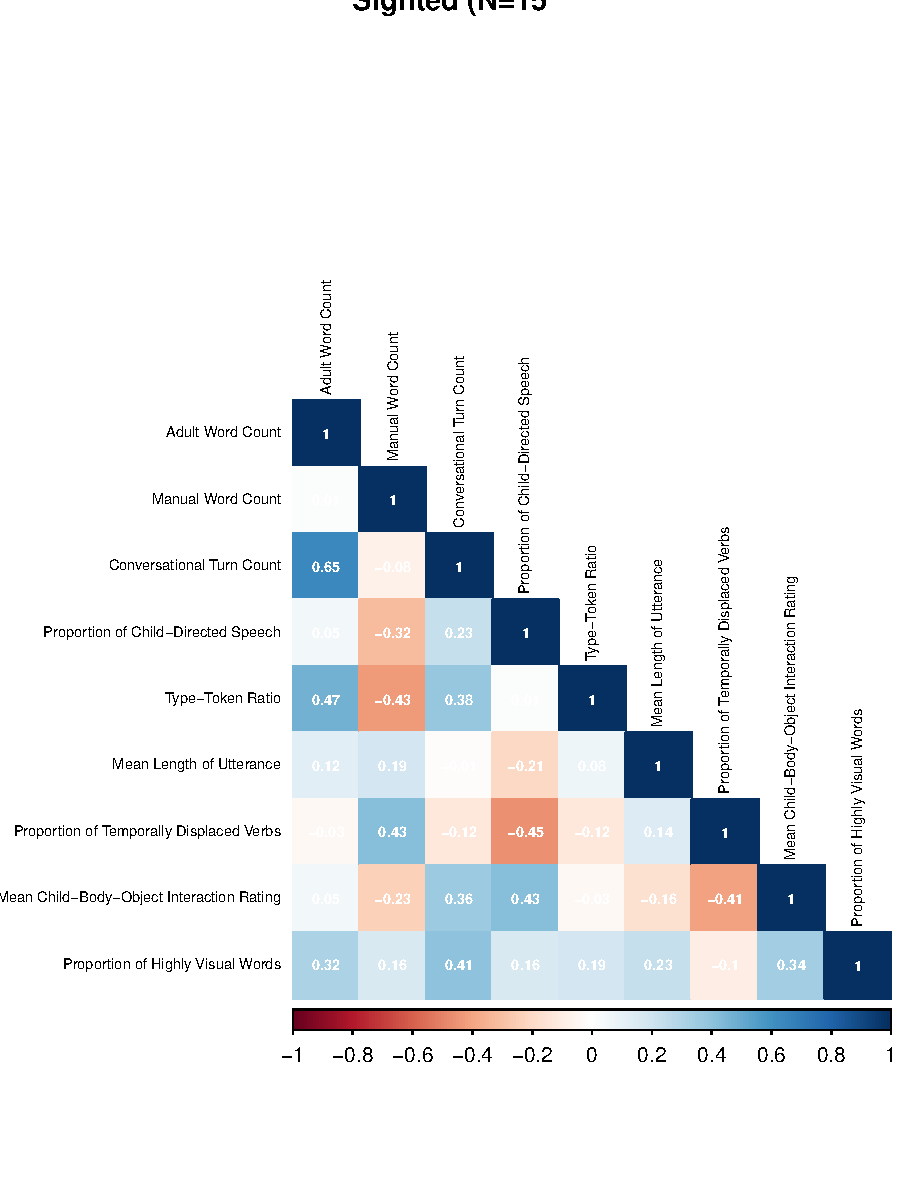
\includegraphics{input_quality_manuscript_files/figure-latex/compare-corrs-2.pdf}

Lastly, we also ran an exploratory analysis testing for patterns among these measures of language input. First, we re-aggregated the language input variables such that each child had a single value for each predictor; this required calculating MLU over child rather than over speaker and giving each child's input a mean child-body-object interaction rating. Next, we generated correlation matrices separately for the blind sample and the sighted sample, using Kendall's Tau correlations; see Figure \ref{fig:compare-corrs}. We then compared correlations among variables across groups. To reiterate, this analysis is purely exploratory and descriptive in nature.

Looking across matrices, we found similarities in how properties of children's language input patterned across groups. To highlight one of the strongest common relationships, in both samples, children who heard more adult words were involved in more conversational turns (\emph{r}\textsubscript{blind} = 0.60, \emph{p}\textsubscript{blind} = .002; \emph{r}\textsubscript{sighted} = 0.65, \emph{p}\textsubscript{sighted} = .001) and had lower type-token ratios (\emph{r}\textsubscript{blind} = -0.69, \emph{p}\textsubscript{blind} \textless{} .001; \emph{r}\textsubscript{sighted} = 0.47, \emph{p}\textsubscript{sighted} = .019). However, we also found some differences, where associations ran in the \emph{opposite} direction: For blind kids but not sighted kids, higher BOI ratings was associated with a greater proportion of temporally displaced verbs; for sighted kids, higher BOI was associated with \emph{less} temporal displacement (\emph{r}\textsubscript{blind} = 0.41, \emph{p}\textsubscript{blind} = .047; \emph{r}\textsubscript{sighted} = -0.41, \emph{p}\textsubscript{sighted} = .047). For blind kids only, proportion of child-directed speech was associated with \emph{lower} proportion of highly visual words (\emph{r}\textsubscript{blind} = -0.30, \emph{p}\textsubscript{blind} = .157; \emph{r}\textsubscript{sighted} = 0.16, \emph{p}\textsubscript{sighted} = .451).

\hypertarget{discussion---ignore-me-for-now}{%
\section{Discussion - ignore me for now}\label{discussion---ignore-me-for-now}}

This study measured language input to young blind children and their sighted peers, using the LENA audio recorder to capture naturalistic speech in the home. We found that across many dimensions of language input, parents largely talk similarly to blind and sighted children, with a few nuanced differences, that we discuss further below.

\hypertarget{quantity}{%
\subsection{Quantity}\label{quantity}}

Across both of measures of language input quantity, one estimated from the full sixteen hour recording (Adult Word Count) and one precisely measured from a 40-minute window of that day (Manual Word Count), blind and sighted children were exposed to similar amounts of speech in the home. Quantity was highly variable \emph{within} groups, but we found no evidence for \emph{between} group differences in input quantity.

\hypertarget{interactiveness-1}{%
\subsection{Interactiveness}\label{interactiveness-1}}

We quantified interactiveness in two ways: through the LENA-estimated conversational turn count, and through the proportion of child-directed speech in our manual annotations. Again, we found no differences across groups in the amount of parent-child interaction. This finding runs counter to previous research; other studies report \emph{less} interaction in dyads where the child is blind (Rowland, 1984; \textbf{perez-pereira2001?}; Andersen et al., 1993; Grumi et al., 2021; Kekelis \& Andersen, 1984; Preisler, 1991;, \textbf{moore1994?}). Using a non-visual sampling method (i.e., our audio recordings) might provide a different, more naturalistic perspective on parent-child interactions, particularly in this population. For one thing, many of these studies (e.g., Kekelis \& Andersen, 1984; Preisler, 1991; \textbf{moore1994?}; \textbf{perez-pereira2001?}) involve video recordings in the child's home, with the researcher present. Like other young children, blind children distinguish between familiar individuals and strangers, and react with trepidation to the presence of a stranger (\textbf{mcrae2002?}; \textbf{fraiberg1975?}); for blind children, this reaction may involve ``quieting'', wherein children cease speaking or vocalizing when they hear a new voice in the home (\textbf{mcrae2002?}; \textbf{fraiberg1975?}). By having a researcher present during the recordings\footnote{Fraiberg (1975) writes ``these fear and avoidance behaviors appear even though the observer, a twice-monthly visitor, is not, strictly speaking, a stranger.'' (pg. 323).} , prior research may have artificially suppressed blind children's initiation of interactions. Even naturalistic observer-free video-recordings appear to inflate aspects of parental input, relative to daylong recordings (\textbf{bergelson2019?}). In these cases, the video camera acts as an observer itself, making participants aware of its presence, limiting participants' mobility, and therefore shrinking the pragmatic scope of possible interactions. Together, these factors could explain why past parent-child interaction research finds that blind children initiate less (Andersen et al., 1993; Kekelis \& Andersen, 1984; \textbf{dote-kwan1995?}; \textbf{troster1992?}; \textbf{moore1994?}), that parents do most of the talking (Andersen et al., 1993; Kekelis \& Andersen, 1984), and that there is overall less interaction (Rowland, 1984; \textbf{nagayoshi2017?}; \textbf{rogers1984?}; \textbf{troster1992?}).

Additionally, a common focus in earlier interaction literature is to measure visual cues of interaction, such as shared gaze or attentiveness to facial expressions (Baird, Mayfield, \& Baker, 1997; Preisler, 1991; \textbf{rogers1984?}). We can't help but wonder: are visual markers of social interaction the right yardstick to measure blind children against? In line with MacLeod and Demers (2023), perhaps the field should move away from sighted indicators of interaction ``quality'', and instead try to understand try to situate blind children's interactions within their own developmental niche, one that may be better captured with auditory- or tactile-focused coding schemes.

\hypertarget{linguistic-features-1}{%
\subsection{Linguistic Features}\label{linguistic-features-1}}

Along the linguistic dimension, we measured type-token ratio and mean length of utterance. Type-token ratio was similar across groups, and in line with type-token ratio in other child-centered corpora (e.g., Newman et al., 2016). However, we found slightly but significantly higher MLU in blind children's language environment. The MLU finding runs counter to common advice: Parents of children with disabilities (including parents of blind children! e.g., (\textbf{familyconnect?}); (\textbf{chernyak?})) are often advised to use shorter, simpler sentences with their children, in order to promote children's understanding. We find instead that the language environments of blind children contain \emph{longer} utterances, which could suggest that consciously modifying your linguistic behavior is difficult for parents. In any case, this advice is not supported by the literature: evidence suggests that longer, more complex utterances are associated with better child language outcomes in both typically-developing children (Hoff \& Naigles, 2002 Mar-Apr) and children with cognitive differences (\textbf{sandbank2016?}).

\hypertarget{conceptual-features-1}{%
\subsection{Conceptual Features}\label{conceptual-features-1}}

The conceptual features of language input feel slipperiest to operationalize. For this analysis, we chose to capture \emph{here-and-now}-ness by measuring the proportion of temporally displaced verbs, the distribution of high vs.~low child-body-object interaction ratings for content words, and the proportion of highly visual words. Relative to other aspects of language input, the conceptual dimension seemed to vary most across groups: though blind and sighted participants were exposed to a similar proportion of highly visual words, blind children heard more displaced verbs and their content words were distributed slightly more to the not-interactable side of the child-body-object interaction ratings.

Furthermore, our exploratory analysis points to potential group differences in the \emph{context} of conceptual information. Blind children's proportion of temporally displaced verbs was inversely correlated with their mean child-body-object interaction rating, whereas sighted children showed the reverse relationship. Could this suggest that when sighted children hear about words that are perceivable or manipulable, it tends to be in the context of co-present objects / events, but when blind children hear about things that can be interacted with, it tends to be related to past/future events? Additionally, while we found that overall, blind and sighted children hear a similar proportion of highly visual words (blue, mirror, rainbow, see), blind children (but not sighted children) who receive \emph{more} child-directed speech seem to receive \emph{less} of this highly visual language. Our present analyses can only hint at potential relationships between these variables at the child level, but as more dense annotation becomes available, we can explore the social and environmental context of conceptual information as it unfolds across discourse.

\hypertarget{patterns-in-language-input-1}{%
\subsection{Patterns in Language Input}\label{patterns-in-language-input-1}}

Before synthesizing any of these differences, we wish to highlight again how much variability there is \emph{within} groups and how much consistency there is \emph{between} groups. One could imagine a world in which the language environments of blind and sighted children are radically different from each other. Our data do not support that hypothesis. Rather, we find far more similarity across groups than difference, and all differences were small in magnitude. This is worth emphasizing and re-emphasizing: across developmental contexts, including, as we show here, visual experience, children's language input is resoundingly similar (\textbf{bergelson2022a?}).

When we zoom into more fine-grained aspects of the input, we found that blind children's language environments contained longer utterances, more temporal displacement, and content words that are harder for children to interact with. Together, these features seem to suggest that blind children's input is more similar to adult-directed speech {[}cite cite cite{]} than sighted children's. This does not seem attributable to differences in addressee: our annotators indicate that there is a similar proportion of child-.vs.adult-directed speech across the two groups.

One explanation for the minimal differences between blind and sighted children's language environments is parents' ability to assess their children's engagement and cognitive level, and thereby tailor their speech accordingly. Sighted parents may be unfamiliar with blind children's signals of interest (Perez-Pereira \& Conti-Ramsden, 1999), and as a result, may respond less often to infants' vocalizations and bids for communication (Rowland, 1984), instead defaulting to more adultlike language. On the other hand, we found between-group differences in how these measures relate to each other. In speech to sighted children, there is a small positive relationship between the amount of child-directed speech and the quantity of highly visual words, but in speech to blind children the opposite is true: parents who use more child-directed speech use \emph{less} highly visual language, which suggests that at least some caregivers are tailoring their language to their child's sensory access when speaking to their child specifically.

However, the evidence that each of these inputs measures differs in its relationship to other measures when examined across these two groups underscores the idea that no feature or its proportion relative to other features can be an indicator of input ``quality'' in and of itself. Speech to children is highly variable; even the dimensions of language input that we attempt to measure are not static in their orientation nor the ways we can operationalize them. And yet, despite all this variation both within and between groups, both blind and sighted children grow up to be competent speakers (Röder et al., 2003; Röder et al., 2000). Future work should explore the relationship between these input measures and the children's own language outcomes; however, given the high variability of all of these variables and their relationship to one another, we do not expect parental input to be at all deterministic of successful language acquisition.

\pagebreak

\hypertarget{references}{%
\section*{References}\label{references}}
\addcontentsline{toc}{section}{References}

\hypertarget{refs}{}
\begin{CSLReferences}{1}{0}
\leavevmode\vadjust pre{\hypertarget{ref-andersen1993}{}}%
Andersen, E. S., Dunlea, A., \& Kekelis, L. (1993). The impact of input: Language acquisition in the visually impaired. \emph{First Language}, \emph{13}(37), 23--49. \url{https://doi.org/10.1177/014272379301303703}

\leavevmode\vadjust pre{\hypertarget{ref-anderson2021}{}}%
Anderson, N. J., Graham, S. A., Prime, H., Jenkins, J. M., \& Madigan, S. (2021). Linking {Quality} and {Quantity} of {Parental Linguistic Input} to {Child Language Skills}: {A Meta-Analysis}. \emph{Child Development}, \emph{92}(2), 484--501. \url{https://doi.org/10.1111/cdev.13508}

\leavevmode\vadjust pre{\hypertarget{ref-baird1997}{}}%
Baird, S. M., Mayfield, P., \& Baker, P. (1997). Mothers' {Interpretations} of the {Behavior} of {Their Infants} with {Visual} and {Other Impairments} during {Interactions}. \emph{Journal of Visual Impairment \& Blindness}, \emph{91}(5), 467--483. \url{https://doi.org/10.1177/0145482X9709100507}

\leavevmode\vadjust pre{\hypertarget{ref-bernsteinratner1984}{}}%
Bernstein Ratner, N. (1984). Patterns of vowel modification in mother\textendash child speech. \emph{Journal of Child Language}, \emph{11}, 557--578.

\leavevmode\vadjust pre{\hypertarget{ref-bigelow1987}{}}%
Bigelow, A. (1987). Early words of blind children. \emph{Journal of Child Language}, \emph{14}(1), 47--56. \url{https://doi.org/10.1017/S0305000900012721}

\leavevmode\vadjust pre{\hypertarget{ref-campbell2022}{}}%
Campbell, E. E., \& Bergelson, E. (2022). Making sense of sensory language: {Acquisition} of sensory knowledge by individuals with congenital sensory impairments. \emph{Neuropsychologia}, \emph{174}, 108320. \url{https://doi.org/10.1016/j.neuropsychologia.2022.108320}

\leavevmode\vadjust pre{\hypertarget{ref-campbell2003}{}}%
Campbell, J. (2003). Maternal {Directives} to {Young Children} who are {Blind}. \emph{Journal of Visual Impairment \& Blindness}, \emph{97}(6), 355--365. \url{https://doi.org/10.1177/0145482X0309700604}

\leavevmode\vadjust pre{\hypertarget{ref-chiesa2015}{}}%
Chiesa, S., Galati, D., \& Schmidt, S. (2015). Communicative interactions between visually impaired mothers and their sighted children: Analysis of gaze, facial expressions, voice and physical contacts. \emph{Child: Care, Health and Development}, \emph{41}(6), 1040--1046. \url{https://doi.org/10.1111/cch.12274}

\leavevmode\vadjust pre{\hypertarget{ref-devilliers1985}{}}%
De Villiers, J. (1985). Learning how to use verbs: Lexical coding and the influence of the input*. \emph{Journal of Child Language}, \emph{12}(3), 587--595. \url{https://doi.org/10.1017/S0305000900006668}

\leavevmode\vadjust pre{\hypertarget{ref-demir2015}{}}%
Demir, Ö. E., Rowe, M. L., Heller, G., Goldin-Meadow, S., \& Levine, S. C. (2015). Vocabulary, syntax, and narrative development in typically developing children and children with early unilateral brain injury: Early parental talk about the "there-and-then" matters. \emph{Developmental Psychology}, \emph{51}(2), 161--175. \url{https://doi.org/10.1037/a0038476}

\leavevmode\vadjust pre{\hypertarget{ref-dirks2020}{}}%
Dirks, E., Stevens, A., Kok, S., Frijns, J., \& Rieffe, C. (2020). Talk with me! {Parental} linguistic input to toddlers with moderate hearing loss. \emph{Journal of Child Language}, \emph{47}(1), 186--204. \url{https://doi.org/10.1017/S0305000919000667}

\leavevmode\vadjust pre{\hypertarget{ref-donnellan2020}{}}%
Donnellan, E., Bannard, C., McGillion, M. L., Slocombe, K. E., \& Matthews, D. (2020). Infants' intentionally communicative vocalizations elicit responses from caregivers and are the best predictors of the transition to language: {A} longitudinal investigation of infants' vocalizations, gestures and word production. \emph{Developmental Science}, \emph{23}(1), e12843. \url{https://doi.org/10.1111/desc.12843}

\leavevmode\vadjust pre{\hypertarget{ref-fenson1994}{}}%
Fenson, L., Dale, P. S., Reznick, J. S., Bates, E., Thal, D. J., Pethick, S. J., \ldots{} Stiles, J. (1994). Variability in {Early Communicative Development}. \emph{Monographs of the Society for Research in Child Development}, \emph{59}(5), i. \url{https://doi.org/10.2307/1166093}

\leavevmode\vadjust pre{\hypertarget{ref-fernald1989}{}}%
Fernald, A. (1989). \href{https://www.ncbi.nlm.nih.gov/pubmed/2612255}{Intonation and communicative intent in mothers' speech to infants: Is the melody the message?} \emph{Child Development}, \emph{60}(6), 1497--1510.

\leavevmode\vadjust pre{\hypertarget{ref-ganea2018}{}}%
Ganea, N., Hudry, K., Vernetti, A., Tucker, L., Charman, T., Johnson, M. H., \& Senju, A. (2018). Development of adaptive communication skills in infants of blind parents. \emph{Developmental Psychology}, \emph{54}(12), 2265--2273. \url{https://doi.org/10.1037/dev0000564}

\leavevmode\vadjust pre{\hypertarget{ref-ganek2016}{}}%
Ganek, H., \& Eriks-Brophy, A. (2016). The {Language ENvironment Analysis} ({LENA}) system: {A} literature review. \emph{Proceedings of the Joint Workshop on {NLP} for {Computer Assisted Language Learning} and {NLP} for {Language Acquisition}}, 24--32. {Umeå, Sweden}: {LiU Electronic Press}.

\leavevmode\vadjust pre{\hypertarget{ref-gergle2004}{}}%
Gergle, D., Kraut, R. E., \& Fussell, S. R. (2004). Language {Efficiency} and {Visual Technology}: {Minimizing Collaborative Effort} with {Visual Information}. \emph{Journal of Language and Social Psychology}, \emph{23}(4), 491--517. \url{https://doi.org/10.1177/0261927X04269589}

\leavevmode\vadjust pre{\hypertarget{ref-gilkerson2018}{}}%
Gilkerson, J., Richards, J. A., Warren, S. F., Oller, D. K., Russo, R., \& Vohr, B. (2018). Language {Experience} in the {Second Year} of {Life} and {Language Outcomes} in {Late Childhood}. \emph{Pediatrics}, \emph{142}(4), e20174276. \url{https://doi.org/10.1542/peds.2017-4276}

\leavevmode\vadjust pre{\hypertarget{ref-goldstein2008}{}}%
Goldstein, M. H., \& Schwade, J. A. (2008). Social feedback to infants' babbling facilitates rapid phonological learning. \emph{Psychological Science}, \emph{19}(5), 515--523. \url{https://doi.org/10.1111/j.1467-9280.2008.02117.x}

\leavevmode\vadjust pre{\hypertarget{ref-grigoroglou2016}{}}%
Grigoroglou, M., Edu, U., \& Papafragou, A. (2016). Are children flexible speakers? {Effects} of typicality and listener needs in children's event descriptions. \emph{Cognitive Science}, 6.

\leavevmode\vadjust pre{\hypertarget{ref-grumi2021}{}}%
Grumi, S., Cappagli, G., Aprile, G., Mascherpa, E., Gori, M., Provenzi, L., \& Signorini, S. (2021). Togetherness, beyond the eyes: {A} systematic review on the interaction between visually impaired children and their parents. \emph{Infant Behavior and Development}, \emph{64}, 101590. \url{https://doi.org/10.1016/j.infbeh.2021.101590}

\leavevmode\vadjust pre{\hypertarget{ref-hadley2017}{}}%
Hadley, P. A., Rispoli, M., Holt, J. K., Papastratakos, T., Hsu, N., Kubalanza, M., \& McKenna, M. M. (2017). Input {Subject Diversity Enhances Early Grammatical Growth}: {Evidence} from a {Parent-Implemented Intervention}. \emph{Language Learning and Development: The Official Journal of the Society for Language Development}, \emph{13}(1), 54--79. \url{https://doi.org/10.1080/15475441.2016.1193020}

\leavevmode\vadjust pre{\hypertarget{ref-hawkins2021}{}}%
Hawkins, R. D., Gweon, H., \& Goodman, N. D. (2021). The {Division} of {Labor} in {Communication}: {Speakers Help Listeners Account} for {Asymmetries} in {Visual Perspective}. \emph{Cognitive Science}, \emph{45}(3), e12926. \url{https://doi.org/10.1111/cogs.12926}

\leavevmode\vadjust pre{\hypertarget{ref-hazan2011}{}}%
Hazan, V., \& Baker, R. (2011). Acoustic-phonetic characteristics of speech produced with communicative intent to counter adverse listening conditions. \emph{The Journal of the Acoustical Society of America}, \emph{130}(4), 2139--2152. \url{https://doi.org/10.1121/1.3623753}

\leavevmode\vadjust pre{\hypertarget{ref-hirsh-pasek2015}{}}%
Hirsh-Pasek, K., Adamson, L. B., Bakeman, R., Owen, M. T., Golinkoff, R. M., Pace, A., \ldots{} Suma, K. (2015). The {Contribution} of {Early Communication Quality} to {Low-Income Children}'s {Language Success}. \emph{Psychological Science}, \emph{26}(7), 1071--1083. \url{https://doi.org/10.1177/0956797615581493}

\leavevmode\vadjust pre{\hypertarget{ref-hoff2003}{}}%
Hoff, E. (2003 Sep-Oct). The specificity of environmental influence: Socioeconomic status affects early vocabulary development via maternal speech. \emph{Child Development}, \emph{74}(5), 1368--1378. \url{https://doi.org/10.1111/1467-8624.00612}

\leavevmode\vadjust pre{\hypertarget{ref-hoff2002}{}}%
Hoff, E., \& Naigles, L. (2002 Mar-Apr). How children use input to acquire a lexicon. \emph{Child Development}, \emph{73}(2), 418--433. \url{https://doi.org/10.1111/1467-8624.00415}

\leavevmode\vadjust pre{\hypertarget{ref-hsu2017}{}}%
Hsu, N., Hadley, P. A., \& Rispoli, M. (2017). Diversity matters: Parent input predicts toddler verb production. \emph{Journal of Child Language}, \emph{44}(1), 63--86. \url{https://doi.org/10.1017/S0305000915000690}

\leavevmode\vadjust pre{\hypertarget{ref-huttenlocher1991}{}}%
Huttenlocher, J., Haight, W., Bryk, A., Seltzer, M., \& Lyons, T. (1991). Early vocabulary growth: {Relation} to language input and gender. \emph{Developmental Psychology}, \emph{27}, 236--248. \url{https://doi.org/10.1037/0012-1649.27.2.236}

\leavevmode\vadjust pre{\hypertarget{ref-huttenlocher2002}{}}%
Huttenlocher, J., Vasilyeva, M., Cymerman, E., \& Levine, S. (2002). Language input and child syntax. \emph{Cognitive Psychology}, \emph{45}(3), 337--374. \url{https://doi.org/10.1016/s0010-0285(02)00500-5}

\leavevmode\vadjust pre{\hypertarget{ref-huttenlocher2010}{}}%
Huttenlocher, J., Waterfall, H., Vasilyeva, M., Vevea, J., \& Hedges, L. V. (2010). Sources of variability in children's language growth. \emph{Cognitive Psychology}, \emph{61}(4), 343--365. \url{https://doi.org/10.1016/j.cogpsych.2010.08.002}

\leavevmode\vadjust pre{\hypertarget{ref-jara-ettinger2021}{}}%
Jara-Ettinger, J., \& Rubio-Fernandez, P. (2021). The social basis of referential communication: {Speakers} construct physical reference based on listeners' expected visual search. \emph{Psychological Review}, No Pagination Specified--No Pagination Specified. \url{https://doi.org/10.1037/rev0000345}

\leavevmode\vadjust pre{\hypertarget{ref-kekelis1984}{}}%
Kekelis, L. S., \& Andersen, E. S. (1984). Family {Communication Styles} and {Language Development}. \emph{Journal of Visual Impairment \& Blindness}, \emph{78}(2), 54--65. \url{https://doi.org/10.1177/0145482X8407800202}

\leavevmode\vadjust pre{\hypertarget{ref-landau1985}{}}%
Landau, B., \& Gleitman, L. R. (1985). \emph{Language and experience: {Evidence} from the blind child} (pp. xi, 250). {Cambridge, MA, US}: {Harvard University Press}.

\leavevmode\vadjust pre{\hypertarget{ref-lavechin2021}{}}%
Lavechin, M., Bousbib, R., Bredin, H., Dupoux, E., \& Cristia, A. (2021). \emph{An open-source voice type classifier for child-centered daylong recordings}. {arXiv}. \url{https://doi.org/10.48550/arXiv.2005.12656}

\leavevmode\vadjust pre{\hypertarget{ref-lucca2018}{}}%
Lucca, K., \& Wilbourn, M. P. (2018). Communicating to {Learn}: {Infants}' {Pointing Gestures Result} in {Optimal Learning}. \emph{Child Development}, \emph{89}(3), 941--960. \url{https://doi.org/10.1111/cdev.12707}

\leavevmode\vadjust pre{\hypertarget{ref-macleod2023}{}}%
MacLeod, A. A. N., \& Demers, C. (2023). Transmitting white monolingual {Anglo-American} norms: {A} concept analysis of {``quality of language''} in parent-child interactions. \emph{Applied Psycholinguistics}, 1--29. \url{https://doi.org/10.1017/S014271642300005X}

\leavevmode\vadjust pre{\hypertarget{ref-macwhinney2019}{}}%
MacWhinney, B. (2019). \emph{{CHAT Manual}}. \url{https://doi.org/10.21415/3MHN-0Z89}

\leavevmode\vadjust pre{\hypertarget{ref-naigles1998}{}}%
Naigles, L. R., \& Hoff-Ginsberg, E. (1998). Why are some verbs learned before other verbs? {Effects} of input frequency and structure on children's early verb use. \emph{Journal of Child Language}, \emph{25}(1), 95--120. \url{https://doi.org/10.1017/S0305000997003358}

\leavevmode\vadjust pre{\hypertarget{ref-newman2016}{}}%
Newman, R. S., Rowe, M. L., \& Bernstein Ratner, N. (2016). Input and uptake at 7 months predicts toddler vocabulary: The role of child-directed speech and infant processing skills in language development. \emph{Journal of Child Language}, \emph{43}(5), 1158--1173. \url{https://doi.org/10.1017/S0305000915000446}

\leavevmode\vadjust pre{\hypertarget{ref-ostarek2019}{}}%
Ostarek, M., Paridon, J. van, \& Montero-Melis, G. (2019). Sighted people's language is not helpful for blind individuals' acquisition of typical animal colors. \emph{Proceedings of the National Academy of Sciences}, \emph{116}(44), 21972--21973. \url{https://doi.org/10.1073/pnas.1912302116}

\leavevmode\vadjust pre{\hypertarget{ref-perez-pereira1999}{}}%
Perez-Pereira, M., \& Conti-Ramsden, G. (1999). \emph{Language {Development} and {Social Interaction} in {Blind Children}}. {London}: {Psychology Press}. \url{https://doi.org/10.4324/9780203776087}

\leavevmode\vadjust pre{\hypertarget{ref-preisler1991}{}}%
Preisler, G. M. (1991). Early patterns of interaction between blind infants and their sighted mothers. \emph{Child: Care, Health and Development}, \emph{17}(2), 65--90. \url{https://doi.org/10.1111/j.1365-2214.1991.tb00680.x}

\leavevmode\vadjust pre{\hypertarget{ref-roder2003}{}}%
Röder, B., Demuth, L., Streb, J., \& Rösler, F. (2003). Semantic and morpho-syntactic priming in auditory word recognition in congenitally blind adults. \emph{Language and Cognitive Processes}, \emph{18}(1), 1--20. \url{https://doi.org/10.1080/01690960143000407}

\leavevmode\vadjust pre{\hypertarget{ref-roder2000}{}}%
Röder, B., Rösler, F., \& Neville, H. J. (2000). Event-related potentials during auditory language processing in congenitally blind and sighted people. \emph{Neuropsychologia}, \emph{38}(11), 1482--1502. \url{https://doi.org/10.1016/S0028-3932(00)00057-9}

\leavevmode\vadjust pre{\hypertarget{ref-romeo2018}{}}%
Romeo, R. R., Leonard, J. A., Robinson, S. T., West, M. R., Mackey, A. P., Rowe, M. L., \& Gabrieli, J. D. E. (2018). Beyond the 30-{Million-Word Gap}: {Children}'s {Conversational Exposure Is Associated With Language-Related Brain Function}. \emph{Psychological Science}, \emph{29}(5), 700--710. \url{https://doi.org/10.1177/0956797617742725}

\leavevmode\vadjust pre{\hypertarget{ref-roseberry2014}{}}%
Roseberry, S., Hirsh-Pasek, K., \& Golinkoff, R. M. (2014 May-Jun). Skype me! {Socially} contingent interactions help toddlers learn language. \emph{Child Development}, \emph{85}(3), 956--970. \url{https://doi.org/10.1111/cdev.12166}

\leavevmode\vadjust pre{\hypertarget{ref-rowe2008}{}}%
Rowe, M. L. (2008). Child-directed speech: Relation to socioeconomic status, knowledge of child development and child vocabulary skill*. \emph{Journal of Child Language}, \emph{35}(1), 185--205. \url{https://doi.org/10.1017/S0305000907008343}

\leavevmode\vadjust pre{\hypertarget{ref-rowe2012}{}}%
Rowe, M. L. (2012). A {Longitudinal Investigation} of the {Role} of {Quantity} and {Quality} of {Child-Directed Speech} in {Vocabulary Development}. \emph{Child Development}, \emph{83}(5), 1762--1774. \url{https://doi.org/10.1111/j.1467-8624.2012.01805.x}

\leavevmode\vadjust pre{\hypertarget{ref-rowe2013}{}}%
Rowe, M. L. (2013). Decontextualized {Language Input} and {Preschoolers}' {Vocabulary Development}. \emph{Seminars in Speech and Language}, \emph{34}(4), 260--266. \url{https://doi.org/10.1055/s-0033-1353444}

\leavevmode\vadjust pre{\hypertarget{ref-rowe2020}{}}%
Rowe, M. L., \& Snow, C. E. (2020). Analyzing input quality along three dimensions: Interactive, linguistic, and conceptual. \emph{Journal of Child Language}, \emph{47}(1), 5--21. \url{https://doi.org/10.1017/S0305000919000655}

\leavevmode\vadjust pre{\hypertarget{ref-rowland1984}{}}%
Rowland, C. (1984). Preverbal {Communication} of {Blind Infants} and {Their Mothers}. \emph{Journal of Visual Impairment \& Blindness}, \emph{78}(7), 297--302. \url{https://doi.org/10.1177/0145482X8407800701}

\leavevmode\vadjust pre{\hypertarget{ref-rubio-fernandez2019}{}}%
Rubio-Fernandez, P. (2019). Overinformative {Speakers Are Cooperative}: {Revisiting} the {Gricean Maxim} of {Quantity}. \emph{Cognitive Science}, \emph{43}(11), e12797. \url{https://doi.org/10.1111/cogs.12797}

\leavevmode\vadjust pre{\hypertarget{ref-senju2013}{}}%
Senju, A., Tucker, L., Pasco, G., Hudry, K., Elsabbagh, M., Charman, T., \& Johnson, M. H. (2013). The importance of the eyes: Communication skills in infants of blind parents. \emph{Proceedings. Biological Sciences}, \emph{280}(1760), 20130436. \url{https://doi.org/10.1098/rspb.2013.0436}

\leavevmode\vadjust pre{\hypertarget{ref-snow1972}{}}%
Snow, C. E. (1972). Mothers' {Speech} to {Children Learning Language} on {JSTOR}. \emph{Child Development}, \emph{43}, 549--565.

\leavevmode\vadjust pre{\hypertarget{ref-soderstrom2021}{}}%
Soderstrom, M., Casillas, M., Bergelson, E., Rosemberg, C., Alam, F., Warlaumont, A. S., \& Bunce, J. (2021). Developing a {Cross-Cultural Annotation System} and {MetaCorpus} for {Studying Infants}' {Real World Language Experience}. \emph{Collabra: Psychology}, \emph{7}(1), 23445. \url{https://doi.org/10.1525/collabra.23445}

\leavevmode\vadjust pre{\hypertarget{ref-tadic2013}{}}%
Tadić, V., Pring, L., \& Dale, N. (2013 Nov-Dec). Story discourse and use of mental state language between mothers and school-aged children with and without visual impairment. \emph{International Journal of Language \& Communication Disorders}, \emph{48}(6), 679--688. \url{https://doi.org/10.1111/1460-6984.12040}

\leavevmode\vadjust pre{\hypertarget{ref-thiessen2005}{}}%
Thiessen, E. D., Hill, E. A., \& Saffran, J. R. (2005). Infant-{Directed Speech Facilitates Word Segmentation}. \emph{Infancy: The Official Journal of the International Society on Infant Studies}, \emph{7}(1), 53--71. \url{https://doi.org/10.1207/s15327078in0701_5}

\leavevmode\vadjust pre{\hypertarget{ref-tomasello1986}{}}%
Tomasello, M., \& Farrar, M. J. (1986). Joint {Attention} and {Early Language}. \emph{Child Development}, \emph{57}(6), 1454. \url{https://doi.org/10.2307/1130423}

\leavevmode\vadjust pre{\hypertarget{ref-uccelli2019}{}}%
Uccelli, P., Demir-Lira, Ö. E., Rowe, M. L., Levine, S., \& Goldin-Meadow, S. (2019). Children's {Early Decontextualized Talk Predicts Academic Language Proficiency} in {Midadolescence}. \emph{Child Development}, \emph{90}(5), 1650--1663. \url{https://doi.org/10.1111/cdev.13034}

\leavevmode\vadjust pre{\hypertarget{ref-urwin1983}{}}%
Urwin, C. (1983). \emph{Dialogue and cognitive functioning in the early language development of three blind children: {Normal} and deficient}. 142--161.

\leavevmode\vadjust pre{\hypertarget{ref-vygotsky1978}{}}%
Vygotsky, L. S., \& Cole, M. (1978). \emph{Mind in {Society}: {Development} of {Higher Psychological Processes}}. {Harvard University Press}.

\leavevmode\vadjust pre{\hypertarget{ref-watkins1998}{}}%
Watkins, S., Pittman, P., \& Walden, B. (1998). The {Deaf Mentor Experimental Project} for young children who are deaf and their families. \emph{American Annals of the Deaf}, \emph{143}(1), 29--34. \url{https://doi.org/10.1353/aad.2012.0098}

\leavevmode\vadjust pre{\hypertarget{ref-weizman2001}{}}%
Weizman, Z. O., \& Snow, C. E. (2001). Lexical input as related to children's vocabulary acquisition: Effects of sophisticated exposure and support for meaning. \emph{Developmental Psychology}, \emph{37}(2), 265--279. \url{https://doi.org/10.1037/0012-1649.37.2.265}

\leavevmode\vadjust pre{\hypertarget{ref-yoshinaga-itano2020}{}}%
Yoshinaga-Itano, C., Sedey, A. L., Mason, C. A., Wiggin, M., \& Chung, W. (2020). Early {Intervention}, {Parent Talk}, and {Pragmatic Language} in {Children With Hearing Loss}. \emph{Pediatrics}, \emph{146}(Supplement\_3), S270--S277. \url{https://doi.org/10.1542/peds.2020-0242F}

\leavevmode\vadjust pre{\hypertarget{ref-yu2012}{}}%
Yu, C., \& Smith, L. B. (2012). Embodied attention and word learning by toddlers. \emph{Cognition}, \emph{125}(2), 244--262. \url{https://doi.org/10.1016/j.cognition.2012.06.016}

\leavevmode\vadjust pre{\hypertarget{ref-yurovsky2016}{}}%
Yurovsky, D., Doyle, G., \& Frank, M. C. (2016). Linguistic input is tuned to children's developmental level. \emph{Cognitive Science}, 6.

\end{CSLReferences}


\end{document}
